\chapter{Introduction}
\label{cap:introduction}

This master’s thesis comprises the research on cognitive impact evaluation of multimodal interfaces for people who are blind. The present chapter introduces the work, presenting the motivation and the problem addressed, as well the objectives. Moreover, it summarizes the approach followed to investigate and answers the research questions raised. The following sections present the contextualization of this study (Section \ref{sec:introduction-context}), the motivation behind the research (Section \ref{sec:introduction-motivation}), the objective and main questions that guided this research (Section \ref{sec:introduction-objective}), the methodology (Section \ref{sec:introduction-methodology}), and, finally, the structure of the sections of this document report (Section \ref{sec:introduction-organization}).

\section{Context}
\label{sec:introduction-context}
According to the ``Disability Overview'' of the World Bank \cite{TheWorldBank2016}, one billion people, or about 15\% of the world's population, experience some form of disability. In 2018, the ``World Health Organization'' \cite{WHO2018Blindness} informs that 1.3 billion people are estimated to have visual disabilities worldwide, of which 36 million are blind.

In face of this huge amount, visual disability has a significant impact on the quality of life of people, including their ability to study, work and to develop personal relationships \cite{Bamac2004}. In this aspect, technologies, such as serious games \cite{Sanchez2015}, have been designed to assist people who are blind to support daily life activities. These technologies work as aids to facilitate their independence, autonomy, and safety. Thus, such technologies help to improve the quality of life of people with visual disabilities and could stimulate and develop several skills, such as cognitive skills \cite{Darin2015}.

Even though there is technology specialized for people who are blind (e.g., serious game \cite{Darin2015}), they are still using applications that are similar to older applications for the sighted population. For example, Battleship was one of the earliest games to be produced as a computer game with its release in 1979 \cite{Hinebaugh2009}. AudioBattleShip, a version for both blind children and sighted playing together came in 2004 \cite{Sanchez2004}. In general, the people who are blind have particular human-computer interaction needs, and the user interface should be suitable for them \cite{Sanchez2015}.

Considering these aspects, there are many efforts to develop accessible multimodal interfaces for people with visual disabilities, especially in multimodal games \cite{Buaud2002}\cite{Grammenos2006}. Despite this effort and in contrast to the visual interface evolution of games and applications for sighted people, interfaces for people who are blind explore other ways to interact with the user. In general, technologies for people with visual disabilities combine different sources of perceptual inputs and outputs. The modes (sources of perceptual inputs and outputs) combined, typically audio and haptics \cite{Sanchez2014a}, and provide multimodal interfaces that enable multimode channels for the combination of different user senses \cite{Sanchez2015}. Although multimodal interfaces could help to improve the learning skills of people with visual disabilities, most of these technologies have been not wholly validated. Mostly, they remain in the prototype phase without being integrated into the people's everyday life \cite{Goria2016}.

Some institutes and laws lay down rules to guarantee the quality of applications that improve the skills of people with disabilities. For children who are blind, there are several applications regarding the specific characteristics for this user \cite{Sanchez2007science}\cite{Sanchez2005c}\cite{Sancheza}\cite{Sanchez2010b}. The \gls{NCLB} Act\footnote{The \gls{NCLB} was a U.S. Act of Congress that supports standards-based education reform based on the premise that setting high standards and establishing measurable goals could improve individual outcomes in education. \acrshort{NCLB} includes incentives to reward schools showing progress for students with disabilities and other measures to fix or provide students with alternative options than schools not meeting the needs of the disabled population \cite{AlicynFerrell2006}.} defines that research in inclusive education must \textit{(a)} utilize the scientific method, \textit{(b)} be replicated in more than one set by more than one investigator, and, \textit{(c)} result in findings that converge to a clear conclusion \cite{AlicynFerrell2006}. These concepts are closely linked to the use of \gls{EBSE} practice, which has a goal:
% TODO contextualizar melhor parágrafo acima


\begin{quotation}
To provide the means by which current best evidence from research can be integrated with practical experience and human values in the decision making process regarding the development and maintenance of software \cite{Kitchenham2004a}.
\end{quotation} 

The \gls{EBSE} could provide a means by which industry practitioners can make rational decisions about technology adoption and a means to increase the acceptability of software-intensive systems that interface with individual users \cite{Kitchenham2004a}. It also provides an input to certification processes of the technology used \cite{Kitchenham2004a}. From this concept, some studies in the area of multimodal applications for people who are blind use Evidence-Based Practice to validate their applications \cite{Sanchez2004,Sancheza} which meets prescribed criteria related to the research design, like quality, quantity, and effect size of supporting research \cite{Dalton2015AssistiveNeeds}\cite{Weber1998}. The cognitive impact evaluation, which has been used as evidence-based in other domains, should, therefore, be able to assess precisely the mechanisms by which people with visual disabilities are developing or enhancing cognitive skills \cite{Darin2015}.

The literature informs that researchers use several methods to describe particular cognitive phenomena. Among them, the controlled experiments, which are formal, rigorous and controlled \cite{Wohlin2000}, are an appropriate solution to measure the cognitive impact \cite{Sternberg2011}. In this point, it is required experiments to verify if the multimodal interfaces of this technologies \cite{Dumas2009} thought for them are effective and how they impact users in cognitive dimensions.

\section{Motivation}
\label{sec:introduction-motivation}

Although essential to ensure safety and real cognitive impact of use, experimentation is not simple. It implies to prepare, conduct and analyze experiments properly \cite{Wohlin2000}. In addition to the inherent challenges of evaluating cognitive impact on multimodal systems, there is a gap of studies proposing instruments and methods for evaluating the cognitive impact in the context of multimodal video games for cognitive enhancement of people who are blind \cite{Darin2015}. Critical issues are frequently neglected during the cognitive evaluation of multimodal video games for people who are blind, such as variables not well defined, poor use of statistical methods, or lacking of treatment in relation to resources and ethical concepts \cite{Mesquita2018CognitiveReview}.

%Furthermore, researchers do not evaluate the cognitive impact, instead they prefer to evaluate system functionality \cite{Mesquita2018CognitiveReview}. As a result, it opens space to contribution in quality of the technology interaction with respect to the cognitive objective.
%\todo[inline]{RETIRADO -- Furthermore, researchers do not evaluate the cognitive impact, instead they prefer to evaluate system functionality \cite{Mesquita2018CognitiveReview}. As a result, it opens space to contribution in quality of the technology interaction with respect to the cognitive objective.}

Frequently, the role of the applications for people who are blind or visually impaired is to help the user cognitive activity. The cognitive purpose assessment is an essential part of software construction for people who are blind \cite{DARIN2018}. To do this, it is necessary a process supporting the objectives in doing experiments correctly \cite{Wohlin2000}, that has a worthy plan and report of experiments in the context.

\citeonline{Kitchenham2004a} presents the scientific known guidelines for evaluating the quality of evidence. They consider:
\begin{itemize}
    \item The strength of the evidence. This has three elements: Level, Quality, and Statistical Precision. Level relates to the choice of study design and is used as an indicator to which bias has been eliminated by design. Quality refers to the methods used by the investigators to minimize bias within the study design. Statistical Precision refers to the P- value or the confidence interval.
    \item Size of effect. The distance of the estimated treatment effect from the null value and the inclusion of clinically important effects in the confidence interval.
    \item Relevance of evidence. The usefulness of the evidence in clinical practice, particularly the appropriateness of the outcome measures used.
\end{itemize}

In addition, the experiment report represents the content that is available to the academic community, and mostly it is the only document by which it is possible to conclude about an experiment and define its quality. The empirical study cannot be distinguished from its reporting \cite{Wohlin2000}. Beyond this, ``published guidelines state the importance of clarifying how the work to be reported relates to existing work (\ldots) , it facilitates drawing a landscape of alternative approaches and relations between different experiments'' \cite{Jedlitschka2007}. Proper actions formulated by the experiment process could be taken to ensure a successful experiment \cite{Wohlin2000}. The patterns to be followed in software engineering are widely used and accepted by community \cite{Freeman2004HeadPatterns}. Thus, having a process, as also guidelines, provides support in setting up and conducting an experiment \cite{Wohlin2000}.


\section{Objective}
\label{sec:introduction-objective}

% objetivo antigo
%{\textbf{to propose an instrument to support the multimodal interfaces impact evaluation for cognitive development and enhancement in people who are blind or visually impaired}}

Besides our motivation, the goal of this research work is \emph{\textbf{to develop a complete review literature to allow the construction of guidelines for multimodal interfaces impact evaluation for cognitive development and enhancement in people who are blind}}. The target audience are IT professionals within the software or hardware environment, as well as encompassing researchers in this area.

Although other software quality characteristics are important, the choice of cognitive impact evaluation results from a gap encountered in the literature. We chose for Guidelines based on the analysis of papers (that we consider reports) from Systematic Literature Review and Grounded Theory process of cognitive impact experiments. Published guidelines state the importance of clarifying how the work to be reported relates to existing work \cite{Jedlitschka2007}. 

As identified by \citeonline{Kitchenham2002PreliminaryEngineering} and \citeonline{Kitchenham2004a}, reporting guidelines are necessary for all relevant kinds of empirical work. The guidelines have to address the needs of different stakeholders (i.e., researchers and practitioners). Moreover, most of the existing guidelines are not explicitly tailored to the specific needs of certain types of empirical studies, e.g., controlled experiments a comprehensive classification of empirical studies \cite{Vinson2008AHumans}. 

To achieve this goal, the state of the art explores the comprehensiveness of cognitive impact experiments and how it is applied in the context . Therefore, the main question of the Systematic Literature Review was \emph{``How is the cognitive impact evaluated on multimodal interfaces for people who are blind?''} For a better understanding, the second goal question was ``What are the challenges regarding impact evaluation on this scenario?'' For this research, we consider assistive technologies that include mobile application, computer software, IoT systems, virtual environments, a video game with multimodal interfaces, or mobile devices.

The Grounded Theory complements the findings in the Systematic Literature Review by doing a qualitative analysis of some points of interest on experiments of cognitive evaluation.

%We found the scenario where the lack of a proper and trustable evaluation is a recurrent situation in the cognitive evaluation process. 
%\todo[inline]{RETIRADO - We found the scenario where the lack of a proper and trustable evaluation is a recurrent situation in the cognitive evaluation process.}

We aim to follow the place requirements on researchers to do an evidence-based empirical \citeonline{Wohlin2000} to a proper cognitive evaluation process, as items described below.

\begin{itemize}
    \item To improve the standard of individual empirical studies and systematic literature reviews of such studies.
    \item To identify outcome measures that are meaningful to practitioners.
    \item To report their results in a manner that is accessible to practitioners.
    \item To perform and report replication studies.
\end{itemize}

In the related literature, some works also propose guidelines for other concepts in the context of accessibility. As an example, the study \cite{Ossmann2006} defines games accessibility guidelines helping developers to design their products with the interface and the parameters adapted to the needs of users with disabilities.

This master's thesis study is part of a research on Human-Computer Interaction focused on interfaces for people who are blind which have been developed for more than 20 years at the University of Chile by the research group on multimodal interfaces for developing cognition in people who are blind. In the timeline of this research, the year 1998 is a milestone due to the paper of \citeonline{Lumbreras1998} which presents a work with 3D acoustic interfaces for the blind.

\section{Methodology}
\label{sec:introduction-methodology}
Our work presents the following methodology to study the cognitive impact evaluation of multimodal interfaces for people who are blind. Each step is summarized to provide the reader with an overview of the research methodology. Hence, the following steps led to the accomplishment of this thesis goal (Figure \ref{fig:methodology}).

\begin{itemize}
\item Step 1: State-of-the-art. A systematic literature review approach \cite{Kitchenham2007} was conducted to review existing primary studies in-depth, describing their results according to the following research questions. The study selection  criteria for the systematic literature review include the papers which present technology with a multimodal interface for people who are blind and that use a method to evaluate the cognitive impact of this interface.
\item Step 2: Qualitative Analysis: A secondary study undertaken to characterize the cognitive impact experiments. The strategy used is to analyze some data retrieved from the systematic literature review and follow the theory \cite{Wuetherick2010}.
\item Step 3: Guidelines Design: the design of guidelines for evaluating the cognitive impact development and enhancement in multimodal interfaces for people who are blind based on results from initial steps and literature of Cognitive Psychology \cite{Sternberg2011,Norman1986a} and \gls{EBSE} \cite{Wohlin2000,Jedlitschka2007,Shepperd2012,AlicynFerrell2006,Shull2008GuideEngineering}. The methodology used to reach the Guidelines is based on evidence by using Systematic Literature Review and Grounded Theory results.
\end{itemize}

 	\begin{figure}[h] 
   	    \captionsetup{width=15cm}%Da mesma largura que a figura
		\Caption{\label{fig:methodology} Research Methodology}
		\UFCfig{}{
			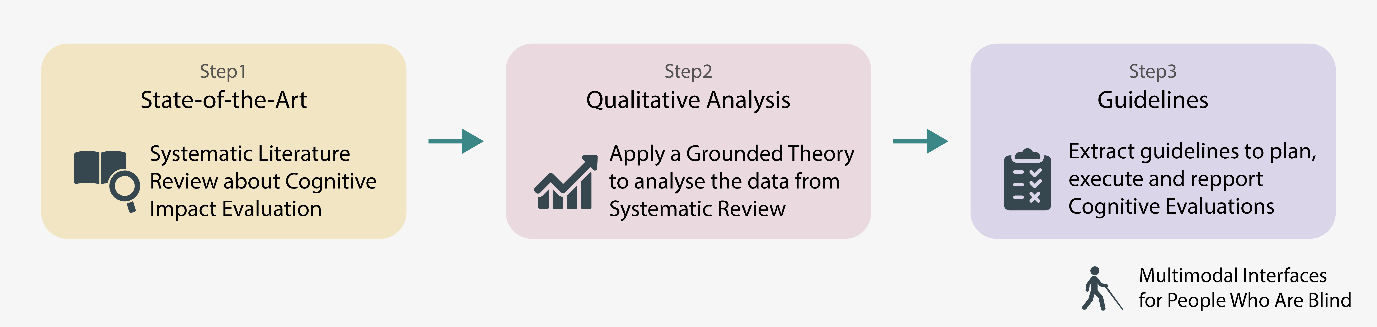
\includegraphics[width=16cm]{figuras/methodology.png}
		}{
			\Fonte{Produced by the author.}
		}	
	\end{figure}


\section{Document Organization}
\label{sec:introduction-organization}

The remainder of the document is organized as follows:
\begin{itemize}
    \item Chapter \ref{cap:background} – Theoretical Background: this chapter describes the bibliography used during the development of this research. This chapter presents the theoretical basis of assistive technology for people who are blind, multimodal interfaces, and \gls{EBSE}.
    \item Chapter \ref{chap:metodologia} – Methodology: this chapter presents the whole process proposed and applied to achieve our objective which is composed of two main steps: The Systematic Literature Review and the Grounded Theory process.
    \item Chapter \ref{chap:resultados} – Results: this chapter presents the results of each step of the methodology that answer the research questions and drives this work. The findings of the literature review and grounded theory process turned into guidelines after the analysis performed. 
    \item Chapter \ref{chap:guidelines} – Guidelines: the findings of the literature review and grounded theory process turned into guidelines after the analysis performed, which  supports cognitive impact evaluation in the context of this study.
    \item Chapter \ref{chap:conclusion} – Conclusion: this chapter presents the conclusion and outlines the main contributions of this research. Moreover, it presents some limitations and some possible paths for future work to continue the research herein presented.
\end{itemize}